\label{timeline}
Given the size of the problem space and that the proposed work will be performed in no more than nine month, we propose to focus on three main contributions:
\begin{inparaenum}[(1)]
\item evaluating and deriving the makespan for a campaign as a set of independent static O(10) workflows with heterogeneous resource requirements provided by ecological and biomolecular sciences use cases on dynamic resources; 
\item offering execution planning capabilities to minimize the makespan of a campaign; and 
\item validating our planning capability by executing the workflows of our use cases and measuring the accuracy of the estimated campaign runtime and planned execution compared to a random plan.
\end{inparaenum}.
In addition, we will explore the requirements to support campaigns with dynamic workflows.

To this end, we propose to achieve the following objectives with an estimation of the time needed:
\begin{enumerate}
    \item Develop a campaign manager prototype, which will derive and execute a plan. Duration 3 months
    \item Implement proposed makespan algorithm for executing a campaign from the ecological sciences. Duration 3 months.
    \item Experimentally measure the performance of the selected makespan algorithm for a scientific campaign. Duration 5.5 months. It overlaps with objective 2 
\end{enumerate}
Figure~\ref{fig:work_plan} shows the Gantt chart of the proposed work.
Subsections~\ref{obj1},~\ref{obj2}, and~\ref{obj3} provide more details as to what will be achieved during each phase of the proposal.

\begin{figure*}[t]
	\centering
	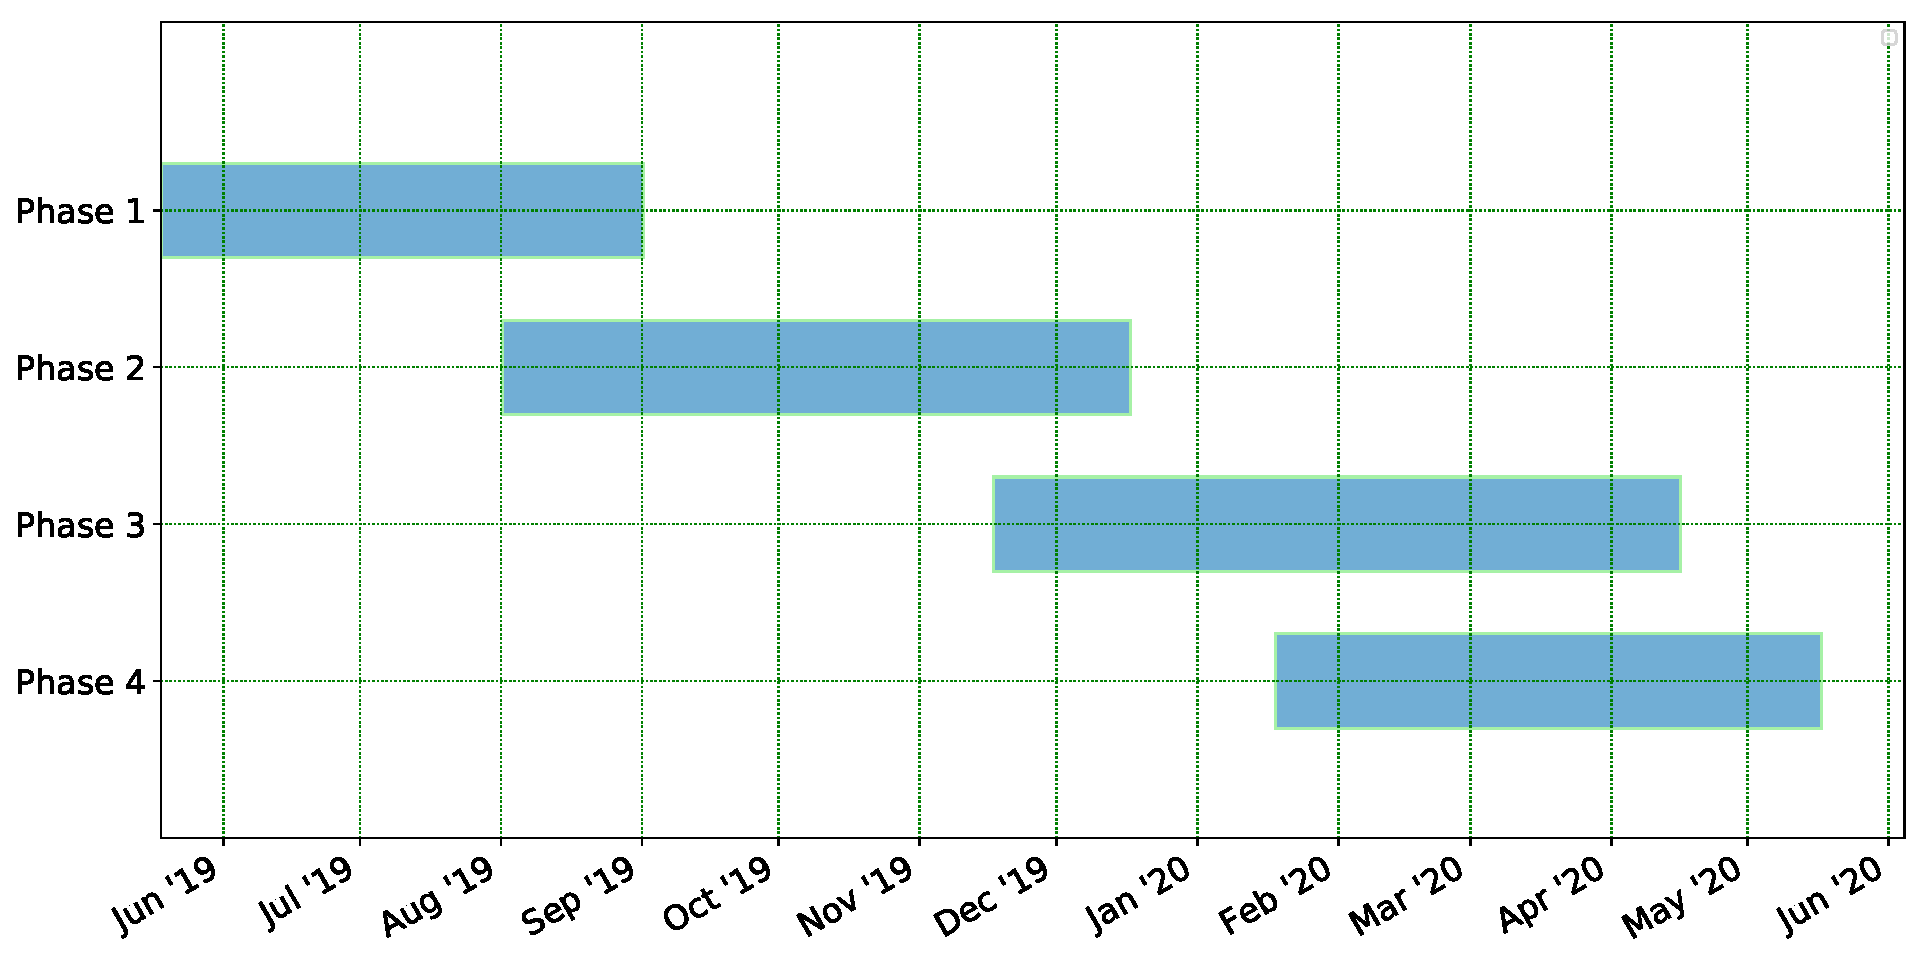
\includegraphics[width=.95\textwidth]{figures/phd_plan.pdf}
	\caption{Planned timeline of proposed research}\label{fig:work_plan}
\end{figure*}

\subsubsection{Phase 1: Design and implementation of a campaign manager}
\label{obj1}

Phase 1 would include design discussions for a prototype of the campaign manager.
Design a prototype is an iterative process, and it will provided the basic functionality of the campaign manager.
Result of these discussions will result to the requirements of the campaign manager and its API.

There are several methods to design a CM.
PanDA~\cite{maeno2008panda} and glideinWMS~\cite{sfiligoi2008glidein} are utilizing a dedicated server to hold all the tasks and schedule them to resources.
Balsam~\cite{salim2019balsam} utilizes a database to hold the campaign and workers are pulling tasks for execution.
DIRAC~\cite{casajus2010dirac} create a set of queues that hold different sized tasks, and use dedicated workers for each queue.
Understanding whether or not existing design approaches fit the requirements of our use cases is necessary to finalize the CM design.

A prototype will be implemented and will provide campaign execution capabilities.
The prototype will be implemented in python and interface with RADICAL-EnTK as its WMF.
Initially, we will assume that the workflows of the campaign are described based on the EnTK's API.
This will allows us to quickly develop the prototype for the campaign manager.
If there is time in phase 1 we will relax this assumption and try to support different methods of describing workflows based on our use cases.
This will require to translate a workflow from any representation to EnTK's.
Furthermore, the planner component should easily allow to support multiple makespan algorithms.
Success of this phase will provide an installable python package. 


\subsubsection{Phase 2: Implementation and performance analysis of makespan algorithm}
\label{obj2}
Phase 2 includes implementing the proposed HEFT algorithm in the prototype, supporting dynamic resources and understand its performance.
Initially, we will implement a random planner, while we extend and implement HEFT to support the campaign.
In addition, we will assume a static campaign with static heterogeneous workflows, executing on static resources.
This will allow us to understand our proposed algorithm, and find its performance compared to a random plan.
Next, we will relax the assumption of static resources and work with dynamic resources and introduce resource dynamicity.

Preliminary experimentation during this phase will provide us with information on whether HEFT can support a campaign execution or not.
In case it does, we will proceed with phase 3 as soon as possible.
Otherwise, we will research algorithms that can support campaign execution and implement them.

\subsubsection{Phase 3: Experimental performance analysis}
\label{obj3}
Phase 3 of the plan includes an experimental performance analysis of the campaign manager for a set of selected use cases.
We will execute campaigns based on our use cases, with and without our campaign manager, for different campaign sizes.
Based on the gathered data, we will measure metrics such as makespan, resource utilization, and overheads to do a performance analysis.
This performance analysis will compare the execution a computational campaign with the prototypical campaign manager and without.
The comparison will provide us with information with the campaign size and characteristics, where a campaign manager should be used.

% ---------------------------------------------------------------------------
% Why
\subsection{Significance and impact of work}
Several scientific campaigns require to execute a large number of workflows several times with different input data or initial conditions. 
The required concurrency to minimize the execution time of the campaign is not necessarily constant and may change based on resource availability. 
The campaign manager suggested in this proposal will be the first to make resource selection decisions for the users. 
This will lead to less time invested by users to make execution decisions about their workflows. 
These decisions will lead to better resource utilization and, as a result, better domain science. 
The empirical performance analysis derived by this work can be used to derive empirical models initial and eventually formal mathematical models.

% ---------------------------------------------------------------------------
% Challenges
\subsection{Challenges/Risks}

We estimate the proposed work, divided into three major phases, to take 9 months 
and we allocate 3 months to account for unforeseen circumstances. We would like 
to keep the committee aware of the following challenges that we see:

\begin{itemize}
	\item Design and Implementation (phase 1) is iterative and special attention needs to be given to the number of iterations against specific objectives, given the timeline.
    \item All experiments performed on HPC systems are subject to variable queue times and may limit the number of experiments performed in phase 2 and 3.
	\item Although the campaign manager will be well tested (80--90\% of the code base will be covered by unit tests) and less susceptible to major changes, RADICAL-EnTK's runtime system, RADICAL-Pilot is known to be less stable and is susceptible to changes as it serves multiple projects.
\end{itemize}